\pdfminorversion=6
\documentclass[12pt]{article}
\usepackage[paper=letterpaper,margin=1in]{geometry}
\usepackage{multicol}
\usepackage[utf8]{inputenc}
\usepackage{graphicx}
\usepackage{color}
\usepackage{float}
\usepackage{hyperref}

% remove lists indentation
\usepackage{enumitem}
\setlist[itemize]{leftmargin=*, itemsep=6pt, topsep=0pt, parsep=0pt}
\setlist[enumerate]{leftmargin=*, itemsep=6pt, topsep=0pt, parsep=0pt}

% discourage single lines at top/bottom of pages
\widowpenalty=10000
\clubpenalty=10000
\displaywidowpenalty=10000

%folder for graphics
\graphicspath{{./figs/}}

% pseudocode
\usepackage[linesnumbered,lined,ruled,commentsnumbered]{algorithm2e}


%%%%%%%%%%%%%%%%%%%%%%%%%%%%%%%%%%%%%%%%%%%%%%%%%%%%%%%%%%%%
\begin{document}
\begingroup
\centering
\LARGE Parallel and Distributed Computing: Homework 1\par
\vspace{10pt}
\endgroup
\noindent
\fbox{
  \parbox{\textwidth}{
    {\bf Objectives} : Use computer simulation to characterize the performance of a shared-memory distributed computing system under assumed workloads. The student is challenged to determine the best number of memory modules connected to a fixed number of processors to process given computational workloads characterized by memory access patterns. Using the C programming language, a computer simulation program is developed and models the computer's resources (processors, memory modules and interconnection network,) models simulated time, models the computational workload, and implements the measuring system (metrology.) Interpreting the results concludes the exercise.}
}    
\vspace{6pt}

%============================================================================
\begin{multicols}{2}
  %\subsection*{System Definition}
  \vspace{-20pt}
  \begin{center}
  \begin{figure}[H]
    %\centering
    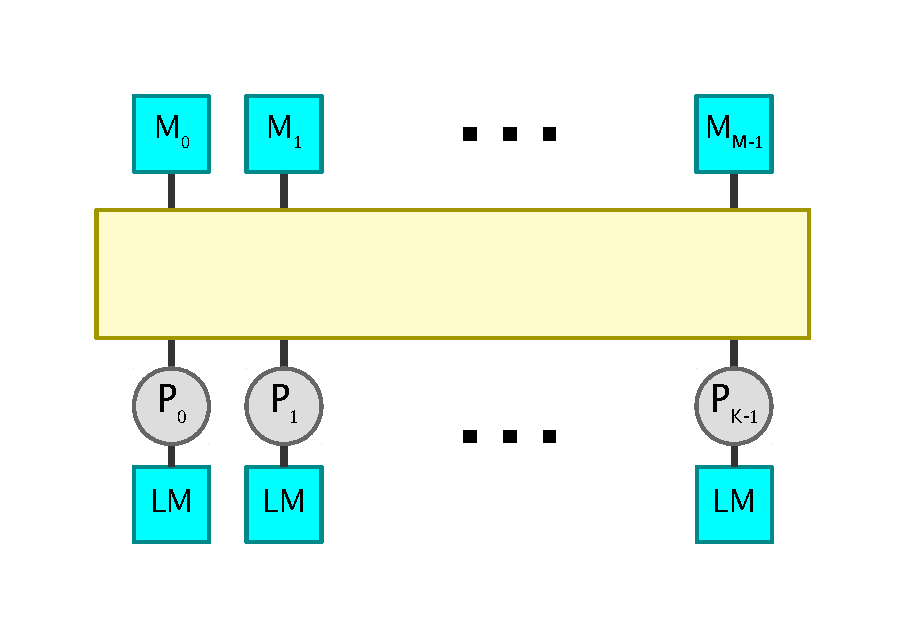
\includegraphics[width=0.5\textwidth]{mimd}
  \end{figure}
  \end{center}
  \vspace{-48pt}
  \paragraph{System Definition:} Consider a system, as the one depicted in the figure above, with $K$ processors and a shared memory subsystem consisting of $M$ single-ported memory modules. Processors and memory modules are interconnected by an interconnection network capable of pairing any processor to any free memory module: at any given time, a non-paired requesting processor connects to one memory module if the module is free, otherwise the processor remains non-paired. A free memory module is one that is not currently paired with any processor. During normal operation, processors run code and request access to data in the shared memory. 
  
  The purpose of this assignment is to use computer simulation to characterize the access time from processors to memory modules under different configurations, namely number of processors and memory modules, and under different workloads exhibiting different memory access patterns, namely the manner in which a concurrent program accesses memory.

  \paragraph{Memory cycles:} For the purposes of simulation, global time is divided into equal successive intervals called ``memory cycles''.

  \paragraph{System processing:} At the beginning of each memory cycle, processors request access to memory modules. Following a priority scheme, each requesting processor is connected to its requested memory module if and only if the module is free. A memory module is free if and only if no other processor has previously been connected to that module during the memory pairing mechanism at the beginning of the current memory cycle.

  Processor access to data is assumed to occur during the remainder of the memory cycle. All memory modules become free again at the end of every memory cycle.

  Processors that are not granted a connection to their requested memory modules wait for the next memory cycle to again request the same memory module.

  At the beginning of the next memory cycle, all processors that were granted access generate a new request while those who waited retry access to their same previously denied memory module.

  \paragraph{Access-Time:} If a processor $x$ is connected to a memory module $y$, no other processor $z$ can connect to $y$ during the same memory cycle. \textbf{Processor $z$ has to wait} and attempt access in the next memory cycle. The number of memory cycles that a processor waits for a memory module will be called ``wait-time''. When a processor accesses a memory module on the first attempt (without waiting), the wait-time is 0. Counting the cycle during which a processor accesses a memory module, the access-time, in units of memory cycles, can be defined as wait-time+1. 
 %The access-time of a processor that has not been yet connected to a memory module is not defined.

   \begin{figure}[H]
    \centering
    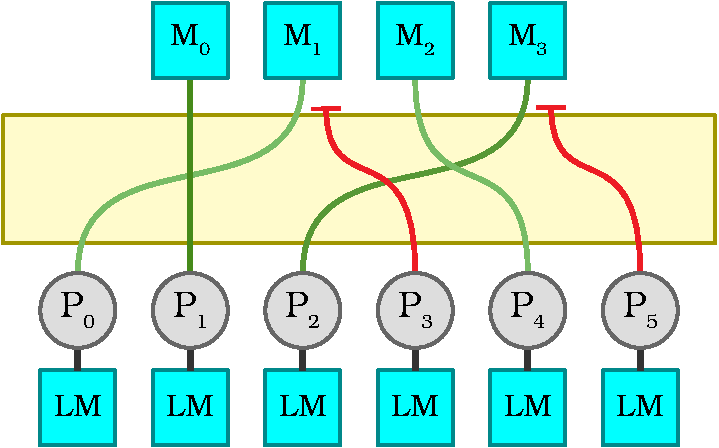
\includegraphics[width=0.37\textwidth]{mimd-example}
  \end{figure}  

  \paragraph{Memory Access Schemes:} To pair processors and memory modules at the beginning of a memory cycle, any non-starving assignment scheme is acceptable. As an example, consider a priority scheme such processors are granted access to memory modules in their natural index order (processors with lower index are granted access first.) In the figure above, this is equivalent to scanning the processing elements from left to right and grant, in that order, memory access to those processors for which the requested memory module is free. In the example of the figure above, $P_3$ and $P_5$ will have to wait to another cycle to gain access to their requested modules. It is clear that this scheme suffers from starvation, some processors may never gain access to requested memory modules. 
  
To fix the problem and avoid starvation, processors can be re-labeled at the beginning of a memory cycle such that the first ``waiting'' processor is re-labeled with index 0 and the remaining processors are cyclicly re-labeled in the natural order. The relabeling can be done dynamically while scanning, or a circular ordered data structure can be kept with a dynamic pointer to the first processor to be considered (which is the first processor with a denied access in the current scan of the processor list.)    


%===========================================================
\subsection*{Assignment}

 You are asked to create a simulator in standard C, without external libraries, to characterize the access-time of processors to memory modules under different configurations and workload characteristics.

  \paragraph{Workload assumptions}
  To represent the memory access demands of a workload, different memory access patterns can be used. Access patterns of an application represent the extent to which locality of reference is present in the workload. For the purposes of this assignment, two distributions of memory requests will be assumed:
  \begin{itemize}
  \item \textbf{Uniform distribution} Each processor issues a random memory module request at the beginning of each memory cycle using a uniform distribution.
  \item \textbf{Normal distribution} In a system with $M$ memory modules, before the main simulation execution, every processor $\pi$ selects one uniformly distributed random memory module $\mu_{\pi}$.
    All subsequent memory requests of processor $\pi$ will be given by $mod(round(X),M)$, where $X$ is a random variable normally distributed with mean $\mu_{\pi}$ and standard deviation $M/6$.
  \end{itemize}



  \paragraph{Computation} Let $S(p,m,d)$ be a system with $p$ processors, $m$ memory modules, and a workload distribution $d$. And let $S_c(p,m,d)$ be the system $S(p,m,d)$ at memory cycle $c$ of its simulation.
  \begin{itemize}
  \item For each number of memory modules $m \in [1,2048]$, a simulation will be run and will be limited to a maximum of $C=10^6$ cycles of $S(p,m,d)$.
 
  \item For each simulation run, you are to compute the time-cumulative average of the access-time for each processor, and the arithmetic average $\bar{W}\left(S_c(p,m,d)\right)$ of all processors' time-cumulative averages. The time-cumulative average of a processor's memory access at cycle $c$ can be computed as the total number of simulated memory cycles $c$ divided by the total number of granted accesses so far.  
  
  \item As it is expected that the average system memory access time $\bar{W}$ settles at some stable value, two termination conditions for the simulation of $S(p,m,d)$ will be considered. 
  
  \begin{itemize}
  \item The system average access time between the current  $\bar{W_c}$ and previous average $\bar{W_{c-1}}$ is less than a certain tolerance $\epsilon$
    %\[Abs\left(\frac{\bar{X}\left\Big(S_{c-1}(p,m_i,d)\right)}{\bar{X}\left\Big(S_c(p,m_i,d)\right)}\right) < 0.0002\]
    \[ 
 Abs  \left( 1- \frac{ \bar{W} \left( S_{c-1}(p,m_i,d) \right) }{ \bar{W} \left( S_c (p,m_i,d) \right) } \right) <  \epsilon 
    \]
    \item or the maximum number of cycles is reached $c=C$
    \end{itemize}
 %\item $m$ is incremented for a new simulation.
  \end{itemize}
    
  \paragraph{Program specification:} Your program will accept 2 command line arguments. You can assume that the given command line arguments will always be correct.
  \begin{itemize}
  \item A positive integer $p$ specifying the number of processors to simulate.
  \item A lowercase character $d$ specifying the distribution of the memory requests with the only possible values \texttt{`u'} (uniform) or \texttt{`n'} (normal).
  \end{itemize}

  Using the code template provided, your programming task is to complete the function \texttt{simulate()} present in the file \texttt{simulator.c} such that it fills the array \texttt{avg\_wait} with the \textbf{last $\bar{W}$ of each one of the 2048 simulations}. Put any needed functions and data structures in \texttt{simulator.c}, which is \textbf{the only source file to be submitted}

  Do not use libraries other than the ones found in GCC, ($9\leq$ GCC version $<12$).

  Finally, while not important for the submission, the \texttt{main.c} program prints the content of your array for easy visualization and plotting.

  \paragraph{Verification of feasibility}
  As long as your code is contained in \texttt{simulator.c}, and the signature of your function is the one we present you in \texttt{simulator.h}, you are free to design your simulation program in any which way you like, however, it suggested to use the following considerations/specifications:
  \begin{itemize}
  \item Using 3 equal size arrays to represent each processors' request, access counter, and priority of connection. Think of this as being a data structure containing $K$ entries, one per each processor, and each entry having, for each processor, a request, access counter, and a priority of connection.
  \item Another array to represent the memory modules. Each element in this array has a 1 if the represented memory module is already connected to a processor or 0 if it is free.
  \item To avoid processing element starvation, it is suggested that you use the cyclic priority index assignment described above to effect processor-memory pairings.
  \end{itemize}



%===========================================================
\subsection*{Report}
Write a report of 2 pages. {\em Do not forget to include your name and student ID number on the top of the first page of your report.} The report must consist of three parts:

\paragraph{Charts} The first page of your report will contain two charts, one each for the assumed uniform and normal distributions. Each chart consists of an X-Y cartesian drawing in which the results of the simulations are plotted. A plot is a curve showing the values on the Y-axis of a variable as a function of values in the X-axis.

\begin{itemize}
  \item In each chart the  X-axis represents the number of memory modules varying from $1$ to $2048$ while the Y-axis represents the values of $\bar{W}$ obtained in the simulations.
  \item Both axis have to be linear (not logarithmic or any other non-linear scale).
  \item Generate one plot (curve) for each fixed number of processors $\{2,4,8,16,32,64\}$. There must be 6 curves per chart.
  Although the data for the plots is generated by your simulator as a set of $\bar{W}$ that can be captured on a file by redirecting the command line output, you can use any available tool to generate the plots, and hence the charts, such as Python/Matplotlib, LibreOffice, Google Sheets, Microsoft Office, etc.
\end{itemize}

\begin{figure}[H]
  \centering
  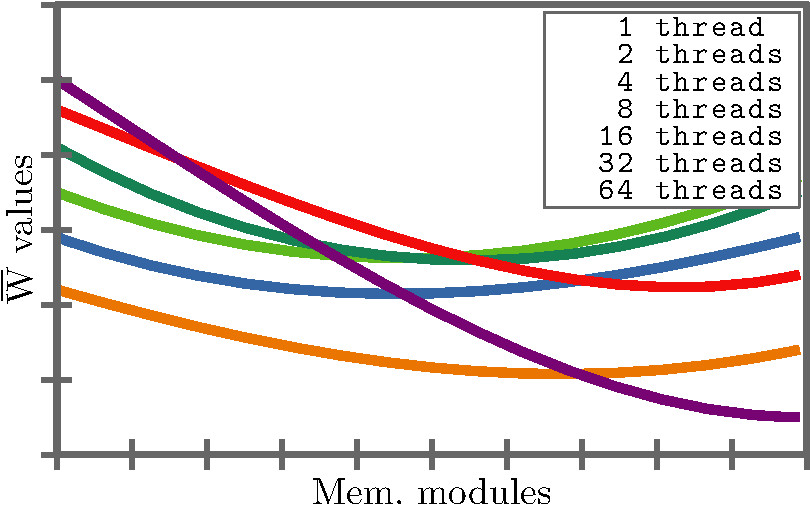
\includegraphics[width=0.45\textwidth]{plot}
\\  {\small (the shape of the curves is not representative.)}
\end{figure}

In summary, parameterizing each chart on the number of processors, six plots (curves) will be superimposed into each chart (as seen in the previous figure).

Include a cropped/zoomed view of the charts if necessary.

\paragraph{Discussion} In the second page, you will include the analysis and interpretation of the obtained results. How does the memory request distribution affects the behavior of the system? If this simulation is in the context of making a decision to buy expensive memory modules for a given number of powerful processors, what would you recommend? Why?

%==========================================================
\subsection*{Submission}
On Canvas (Main Space or Assignments), submit \textbf{one} zip file named \texttt{hw1.zip}, containing \textbf{exactly 3 files}. Make sure the zip file does \textbf{not} include sub-directories (as Mac's default compression tool does) or extra files:
\begin{enumerate}
\item \texttt{simulator.c}: The well commented C source code file implementing the function \texttt{simulate()}.
\item \texttt{report.pdf}: The digitally produced report of 2 pages.
\item \texttt{team.txt}: Text file with two lines containing the UCINetID and name of each student:\\
  \texttt{<UCINetID\_1> <firstName> <lastName>}
\end{enumerate}
\end{multicols}
\end{document}
